\section{Drive App Tab}

The main option to interact with Drive is clicking on the Drive tab.
This click can have two different behaviours: 
\begin{itemize}
    \item{everything is fine and the main drive view(Figure \ref{fig:view}) will be opened}
    \item{cannot communicate with drive and the error view(Figure \ref{fig:errUnreachable}) will be opened}
\end{itemize}

When the tab is clicked for the first time, a request with the current zimbra user credentials is sent to drive and 
that request creates or loads the current user drive space. Then this space is shown in the drive view.\\
The drive view is composed by the left sidebar with the complete tree of the folders 
and the main view with the content of the current folder. On load the current folder is the root folder by default.\\
\begin{figure}[htbp,!h] 
\centering 
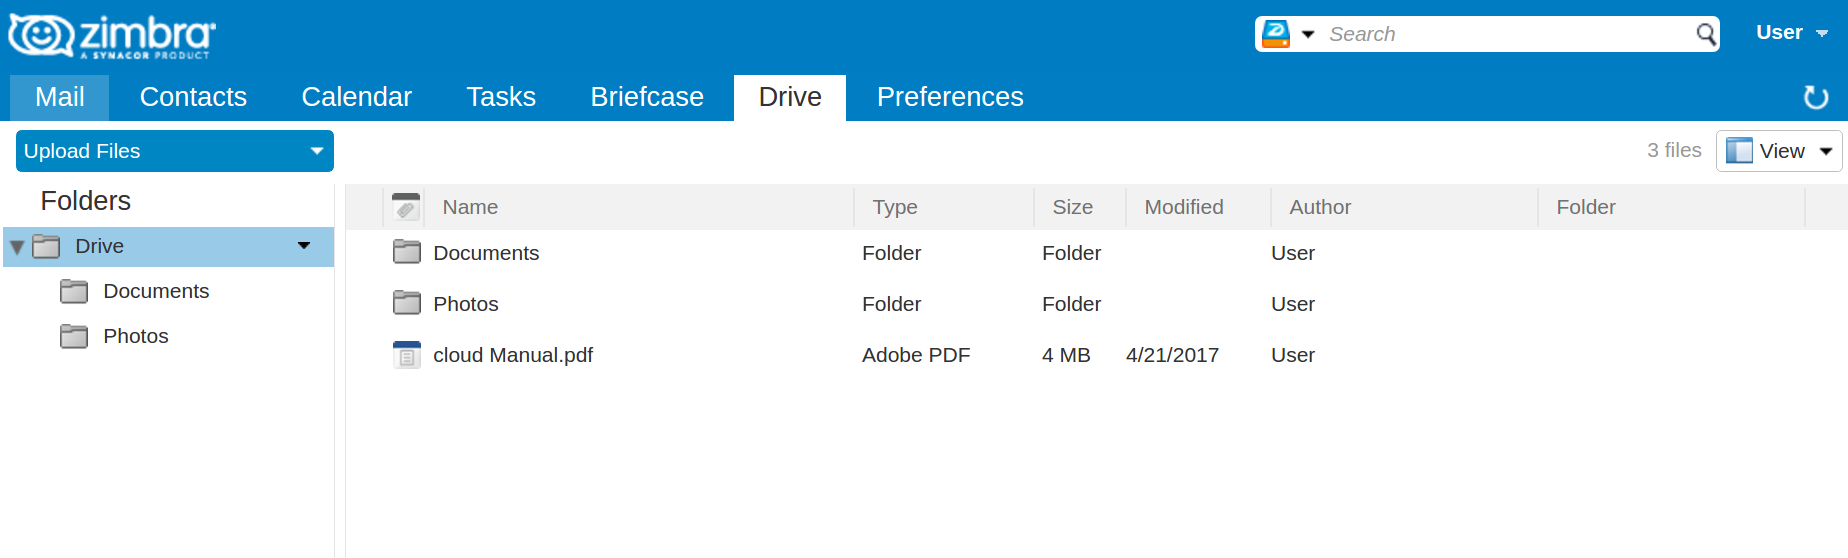
\includegraphics[scale=0.25]{\srcPath/images/ZD-view.png} 
\caption{Main View} 
\label{fig:view}
\end{figure}
\\

\subsection{Navigate through Folders}
The left sidebar let user opens selected folder by left single-clicking on it. 
The selected folder becomes highlighted and the content is shown in the main view.\\
Only the current folder content composed by files and folders is shown in the main view;
the folders can be double-clicked in order to change folder to the selected one.\\
It's possible to refresh the current drive view clicking on refresh icon in the top right corner, under the user account name(see Figure \ref{fig:view}).

\subsection{Error View}
When the error view is shown(Figure \ref{fig:errUnreachable}), it means that it's not possible for zimbra to communicate with the drive and
only a sysadmin can fix the server configuration.\\
The user can retry without refreshing the zimbra using the linked button.
\begin{figure}[htbp,!h] 
\centering 
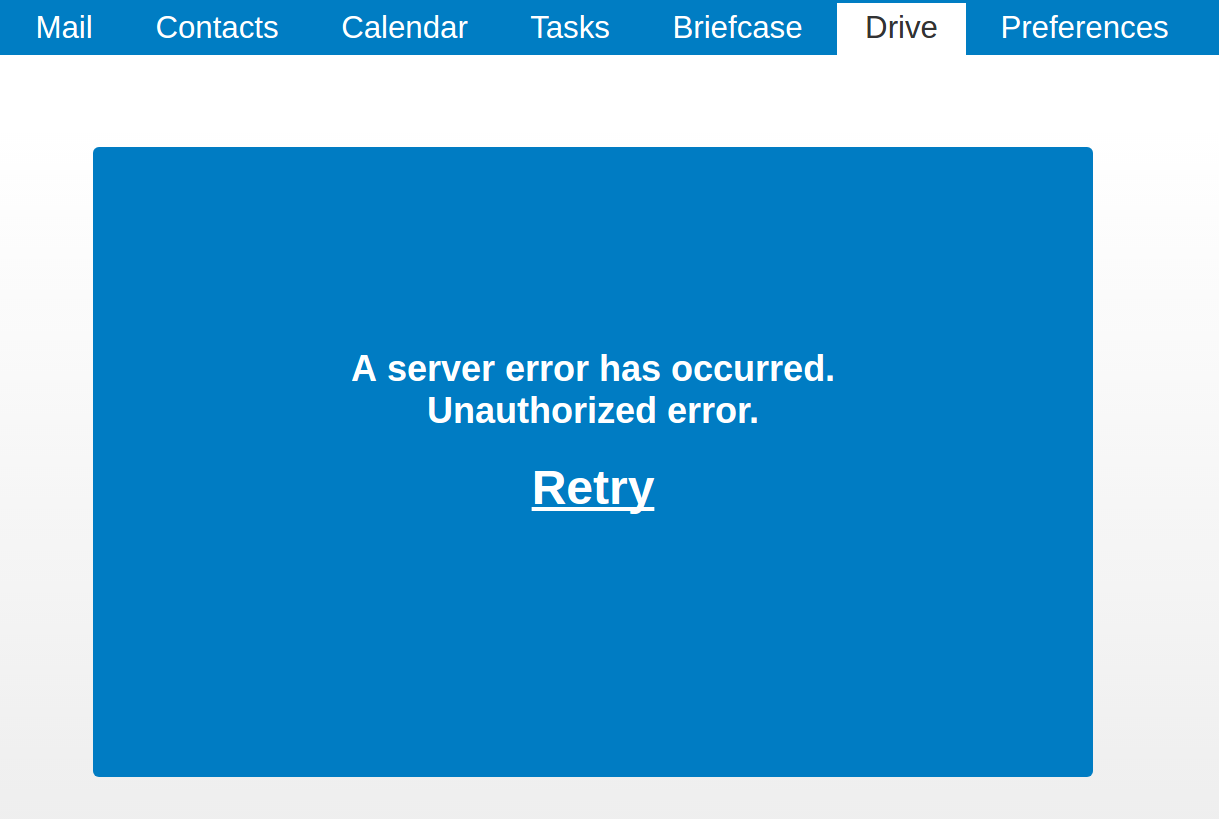
\includegraphics[scale=0.18]{\srcPath/images/ZD-errorUnreachable.png} 
\caption{Error View} 
\label{fig:errUnreachable}
\end{figure}
